\chapter{Proposed Solution}

\section{Doors Detector}

The main objective of this thesis is to propose a door detection module that is able both to find doors within RGB images and to understand their status (open or closed). We reduce these problems to a precise Computer Vision's task: object detection. Today, the most relevant techniques used in Computer Vision are based on the power of Deep Learning. This is because the doors detector is based on DETR \cite{detr}, a novel end-to-end deep module based on Tranformers. Before talking about DETR and how it is used to detect doors, we review the most relevant aspects in the theory of Deep Learning.

\subsection{Deep Learning Review}

Deep Learning is a sub-field of Machine Learning, that is the study of computer algorithms that can improve automatically through experience and by the use of data. We define some important aspect of Machine Learning before talking about the proposed approach to detect doors. Machine Learning is a powerful technique suitable when it is not feasible to develop a standard algorithm to solve a difficult task. A \textit{learning algorithm} uses sample pairs of training data to create a model, also called predictor, that is able to classify other unseen data. The first important aspect for a machine learning problem is the dataset. Typically, a dataset is composed by pairs of data taken from two different sets: the \textit{data domain} and the \textit{label set}.

\begin{definition}[Data domain]
	We use $X$ to denote the set of all possible data points for a given learning problem. Each data point is composed by features. In some cases, the features are encoded as vectors of real numbers. Such a vector representation is \textit{natural} whenever the data consist of homogeneous quantities, like pixels in an image or words' frequencies in a document. A data point is denoted as $x \in X$ and it is defined as a vector of feature $x = (x_1, ..., x_d)$.
\end{definition}

\begin{definition}[Label set]
	We use $Y$ to denote the set of all possible labels for a data point of a given learning algorithm. For a classification problem, the label set is typically finite and small (such as $Y = \{sport, policies, business\}$ for a documents categorization task).
\end{definition}

In a \textit{supervised} learning problem, the data point are tagged with their respective ground truth labels. In particular, the dataset's entries are pairs $p = (x, y)$, where $x \in X$ is a data point and $y \in Y$ is the label assigned to it. A \textit{supervised} learning algorithm is a technique that aims to build a model learned from a \textit{training set}. This paradigm is called \textit{learning by examples}. An example is a pair $p=(x, y)$ (where $x$ is a data point represented by a feature vector and $y$ is its ground truth label) and the training set is composed by a series of examples $S=\{(x_1, y_1), ..., (x_m, y_m)\}$. A \textit{supervised learning algorithm} for \textit{learning by examples} receives a training set and outputs a learned model.

\begin{definition}[Model]
	A model is a function $f:X \to Y$ that maps data points to labels.
\end{definition}

The training examples come from some generally unknown probability distribution and the goal of a learning problem is to infer a function that approximates this distribution (or makes a generalization of it) to produce sufficiently accurate predictions in new cases. In order to estimate the predictive power of a model, we typically use a \textit{test set}. This is a set of examples $T=\{(x_1', y_1'), ..., (x_n', y_n')\}$ that the learning algorithm does not have access during the training phase. Each pair in the \textit{test set} are fed into the model in order to measure the goodness of each prediction compared with the ground truth label. This measure is computer using the \textit{loss function}.

\begin{definition}[Loss function]
	A loss function $\ell(y, \hat y)$ measure the discrepancy between the predicted label $\hat y$ and the ground truth label $y$. For a correct prediction, $\ell (y, \hat y) = 0$.
\end{definition}

A way to train a learning model is the Empirical Risk Minimization (ERM) approach. The test set allows to determine the predictive power of a learned model on unseen new data. To measure the goodness of a predictor, we can calculate the \textit{test error} over a test set $S$. 

Given a loss function $\ell$, the test error is
\begin{equation}
\frac{1}{n} \sum_{t=1}^{n}\ell(y_t', f(x_t'))
\end{equation}
where the $n$ is the test set's cardinality ($n = |S|$), $y_t'$ is the ground truth label of the f-th test example and $f(x_t')$ returns the predicted label from the t-th data point. Since the test set is disjoint from the training set, ERM offers a theory to design learning algorithms that generate predictors with a low test error considering only the training set. ERM assumes that the \textit{training error} (the error computed over a training set $T$) of a predictor is directly correlated to its test error. The training error is given by 

\begin{equation}
\hat \ell(f) = \frac{1}{m} \sum_{t=1}^{m}\ell(y_t, f(x_t))
\end{equation}
where the $m$ is the test set's cardinality ($m = |T|$).



\begin{definition}[Empirical risk minimization] 
	Let $\mathcal{F}$ a set of predictors and $\ell$ a loss function. The empirical risk minimizer (ERM) is the learning algorithm that outputs some predictor in $\mathcal{F}$ minimizing the training error
	
	\begin{equation}
	\hat f \in \argmin_{f \in \mathcal{F}} \hat \ell(f).
	\end{equation}
	The notation $\in$ denotes there could be multiple $f \in \mathcal{F}$ that minimizing the training error.
\end{definition}

The ERM algorithm fails when no predictors in $\mathcal{F}$ have a low test error, in particular when 

\begin{equation}
	\min_{f \in \mathcal{F}} \frac{1}{n} \sum_{t = 1}^{n} \ell(y_t', f(x_t'))
\end{equation} 
is high. The two main ways of failing for a generic learning algorithm are:
\begin{itemize}
	\item \textbf{underfitting:} when a learning algorithm tends to outputs predictors whose test and training errors are high and closed to each other. This situation could depend on the training test size: if it is too small it can not represents well the data points' distribution or $\mathcal{F}$ (the set of the possible predictors) are too large with respect the training set dimensions. Another reason that causes underfitting is the cardinality of $\mathcal{F}$. If the set of the possible predictors is small, there could not be a subset of them with small test error. This means that the learning algorithm is not complex enough to output good learned models. In other words, when a model underfits it is not able to generalize well the problem, failing to classify example from both training and test sets;
	\item \textbf{overfitting:} when a learning algorithm tends to output predictors whose training error is low (or it tends to zero) and test error is high. In this situation, the predictors produced by a learning algorithm learn too much from the training data and, as a result, are unable to produce good predictions on new data. This means that those predictors do not generalize the problem, but are specialized in dealing only with the data using during the training phase.
\end{itemize}

When $A$ is a ERM learning algorithm and the size $m$ of the training set is fixed, we should expect overfitting when $\log_2|\mathcal{F}| \gg m$, so the set of possible predictors is to large with respect to the training set's size. On the other hand, when $\log_2|\mathcal{F}| \ll m$ we should expect underfitting.

Deep Learning is a subfield of Machine Learning based on \textit{neural networks}. This learning algorithm is inspired by the information processing and distributed communication of biological brains. Neural networks (NNs) are a large and complex class of predictors, based on artificial neurons.

\begin{definition}[Neuron]
	An artificial neuron is a mathematical function inspired from biological neuron and it represents the elementary units in an artificial NN. The matematical function implemented by a neuron is $g(x) = \sigma(\omega^\intercal \cdot x)$, where $\sigma$ is the activation function, $\omega$ is the weight vector of learnable parameters,and $x$ is the input vector of the neuron. This means that each input is separately weighted and the sum is passed through a non-linear function. The activation function usually have a sigmoid shape and often it is monotonically increasing, continuous, and bounded. 	
\end{definition}

Artificial neural network are composed by a series of simple predictions made by neurons. The adjective ``deep'' in Deep Learning refers to the use of multiple layers in NNs. The most simple model of neural network is feedforward NN. 

\begin{definition}[Feedforward neural network]
A feed forward neural network computes functions of the from $f : \R^d \to \R^n$. Its structure is a directed acyclic graph $G = (V, E)$, in which $V$ is the set of nodes (neurons) and $E$ is the set od edges that connects the neurons. The vertices in $V$ are divided into three subgroups: $V = V_{in} \cup V_{hid} \cup V_{out}$, where $V_{in}$ (with $|V_{in}| = d$, the feature space's dimension) are the input nodes which have no incoming edges, $V_{out}$ (with $|V_{out}| = n$, the number of labels) are the output nodes which have no outgoing edge, and $V_{hid}$ are the hidden nodes, which have both incoming and outgoing edges.
\end{definition}

The most simple form of feedforward neural network is the multi layered perceptron (MLP), in which the nodes of $V$ can be partitioned in a sequence of layers such that each node of a layer has incoming edges only from
nodes in the previous layer and outgoing edges only to nodes of the next layer.  The layers containing the hidden nodes are called hidden layers. 

\begin{figure}[h!]
	\centering
	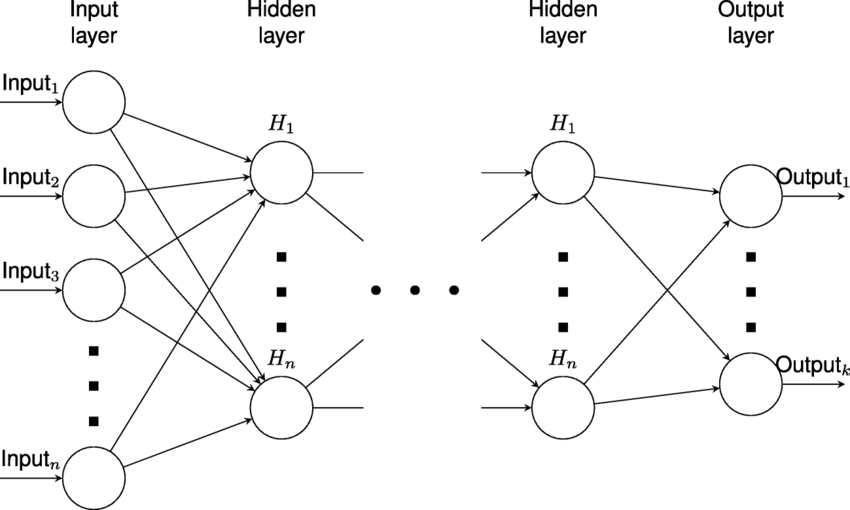
\includegraphics[width=0.9\linewidth]{images/mlp.png}
	\caption{An example of feedforward neural network, with $d$ input nodes and $n$ output nodes. In this example, the connectivity between layers is complete (there are no missing edges).}
\end{figure}

The learnable parameters are the weights assigned to the edges between neurons. 
A parameter $\omega_{i,j} \in \R$ (called weight) is associated with every edge pair $(i, j) \in E$.  We use $W$ to denote the $|V | \times |V |$ weight matrix, where $(i, j) \notin E$ implies $\omega_{i,j} = 0$. The graph $G$, the weights matrix
$W$, and the activation function $\sigma$ define the function $f = f_{G,W,\sigma}$ computed by the network.  Note that when $n = 1$ (one output node) and $|V_{hid}| = 0$ (no hidden nodes), then $F_{G,\sign}$ only contains linear classifiers of the form $f(x) = \sign(\omega^\intercal \cdot x)$. The training of neural networks is not trivial. The most natural approach for training a model in $\mathcal{F}_{G,\sigma}$ is ERM.
Unfortunately, this method could not efficiently applied to neural networks. 

\begin{theorem}
	For every integer $k \geq 3$, let $G$ be a network with $d$ input nodes, a single hidden layer containing $k + 1$ nodes (one of which has constant value 1), and a single output node. Then the problem of minimizing the zero-one loss training error in $\mathcal{F}_{G,\sign}$ is NP-hard. 
\end{theorem}

The models considered by this theorem are simplified neural networks to solve a \textit{binary classification} task using the zero-one loss (equation \ref{formula:zero-oneloss}) with a single hidden layer composed by four or more neurons. 

\begin{equation}
	\label{formula:zero-oneloss}
	\ell(y, \hat y) = 
	\begin{cases}
	0 & \text{if $y = \hat y$} \\
	1 & \text{if $y \neq \hat y$}
	\end{cases}
\end{equation}

This theorem demonstrates the inefficiency of ERM for a simple NN. This means that this theorem is true even for more complex neural networks and different tasks. ERM remains NP-hard even when $\mathcal{F}_{G,\sign}$ contains only linear classifiers (i.e., $G$ has no hidden nodes). However, while the cause of NP-hardness in linear models was the non-convexity of the loss function (zero-one loss in this case), in multi-layered neural networks the problem is inherent to their structure. The key observation is that the presence of hidden nodes in NN makes the loss function $\ell_t$ over a example $(x_t, t_t)$ non-convex in the weights matrix $W$ even when $\ell(x, y)$ is convex for all $y$. In general, the problem of minimizing a non-convex function is computationally intractable.  

This is because NNs are successfully trained using algorithms that reduce the training error without any mathematical guarantee on the solution's quality. The training procedure starts with a forward propagation of the training examples in the neural network. After that, the outputs are used to quantify how good the predictions are and the error are back-propagated in the network using a descent algorithm. The standard training algorithm for NNs is stochastic gradient descent (SGD):

\begin{equation}
\omega_{i, j} \leftarrow \omega_{i, j} - \eta_t \frac{\partial\ell_{Z_t}(W)}{\partial\omega_{i, j}} \quad \quad (i, j) \in E,
\end{equation}
where $Z_t$ is the index of a random training example and $\eta$ is an hyper-parameter that controls the step size (also called learning rate). The main idea is to calculate the partial derivative of the loss function, calculated on a training data point $t$ and the current NN status (described by the weights matrix $W$), over all the learnable parameters to adjust their values. In order to speed up convergence, the training samples can be grouped in mini-batches. Because the training error is a non-convex function of $W$, the SGD algorithm essentially finds only local minima of the training error. The procedure to perform gradient descent on feedforward NNs is known as \textit{error back-propagation}. 

\subsection{DETR}

The doors detector proposed by this thesis is based on DETR \cite{detr} (DEtection TRansformer), a novel deep approach to perform object detection. In DETR, object detection problem is modeled as a direct \textit{set prediction}, making the detection pipeline a simple end-to-end unified architecture. Modern detectors address this set prediction in an indirect way using hand crafted algorithms based on a large set of proposals \cite{yolo} or anchors \cite{focalloss}. Their performances are significantly influenced by these post-processing steps to collapse near-duplicate predictions, like non-maximum suppression or anchor generation. The first important aspect the architecture (explained in Sec. \ref{sec:detrarchitecture}). DETR uses a Transformer to finds complex relationships between features extracted in the same image. In this way, the model reasons about the whole image context without considering any form of prior knowledge about the task. The second important aspect to address the set prediction problem are the loss functions (described in \ref{sec:detrlosses}). DETR uses a set loss function which performs bipartite matching between predicted and ground-truth objects.

\subsubsection{DETR Architecture}
\label{sec:detrarchitecture}
The architecture of DETR (reported in Fig. \ref{fig:detrarchiecture}) consists on three main components: a convolutional neural network (CNN) backbone for features extraction, an encode-decoder transformer to capture the relationships between the extracted features, and a simple feed forward network (FFN) that makes the final detection prediction (the coordinates of the bounding boxes and their relative labels).

\begin{figure}[h!]
	\centering
	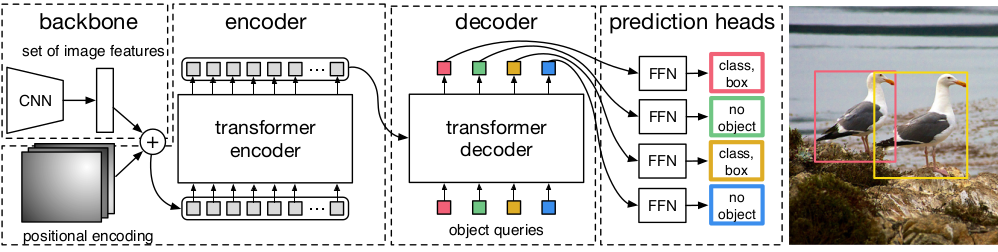
\includegraphics[width=\linewidth]{images/detrarchitecture.png}
	\caption{The architecture of DETR. It uses a conventional CNN backbone to learn a 2D representation of an input image. Then, this representation is flattened and encoded before being passed into the transformer encoder. The transformer decoder then takes as input a small fixed number of learned positional embeddings, called \textit{object queries}, and additionally attends to the encoder output. Finally, each output embedding of the decoder is processed by a  feed forward network (FFN) that predicts either a detection (class and bounding box) or a ``no object'' class. Image from \cite{detr}.}
	\label{fig:detrarchiecture}
\end{figure}

\paragraph{CNN Backbone} The first element in DETR's architecture is a CNN backbone.  Ideally, any backbone can be used depending upon the complexity of the task to provide low dimensional representation of the image extracting features from it. Starting from the initial image $x_{img} = \R^{3\times H_0\times W_0}$ (with 3 color channel and dimension $H_0$, $W_0$), a conventional CNN backbone generates a lower-resolution activation map $f \in \R^{C×H×W}$. Typical values used in this paper are $C = 2048$ and $H, W = \frac{H_0}{32}, \frac{W_0}{32}$. 

The authors uses ResNet (residual network) \cite{resnet} as CNN backbone, a neural network that solve the issue of vanishing gradient. This problem makes deeper neural network more difficult to train and optimize: when network depth increasing, accuracy gets saturated and then degrades rapidly. This unwanted situation is called \textit{degradation} (of training accuracy). Unexpectedly, such degradation is not caused by overfitting, and adding
more layers to a deep model leads to higher training error. The authors address the degradation problem by introducing a \textit{deep residual learning} framework, commonly called ResNet. The proposed method is based on the insight that a few overlapping layers can fit a residual mapping instead of directly fitting a desired underlying mapping. This principle is formalized as follow. Let $\mathcal{H}(x)$ be the desired underlying mapping fit by a few stacked layers (not necessarily the entire net), where $x$ denotes the inputs of the first layer. Since multiple non-linear layers can approximate  non-linear functions, then  the same layers can approximate the residual functions $\mathcal{H}(x) - x$. The authors let these layers approximate a residual function
$\mathcal{F}(x) := \mathcal{H}(x) - x$:  now the original function becomes
$\mathcal{F}(x)+x$. The authors hypothesize that it is easier to optimize the residual mapping than to optimize the original, unreferenced mapping.  If the optimal function is closer to an identity
mapping than to a zero mapping, it should be easier for the
solver to find the perturbations with reference to an identity
mapping, than to learn the function as a new one. This means that subsequent blocks in our network are thus responsible for fine-tuning the output of a previous block, instead of having to generate the desired output from scratch.

\begin{figure}[h!]
	\centering
	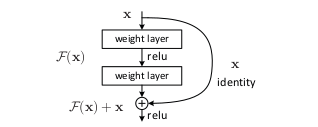
\includegraphics[width=0.6\linewidth]{images/residualblock.png}
	\caption{Residual learning: a building block. The formulation of $\mathcal{F}(x)+x$ can be realized with a ``shortcut connection'', that skips one or more layers. Image from \cite{resnet}.}
	\label{fig:resblock}
\end{figure}

\paragraph{Transformer Encoder-Decoder} The second part of DETR is a Transformer \cite{transformer}, a novel sequence-to-sequence (Seq2Seq) architecture that transforms a given sequence of elements, such as the sequence of words in a sentence, into another sequence. Seq2Seq models are particularly useful for natual language process tasks (NLP), text classification, machine translation and
question answering. Among their salient benefits, Transformers enable modeling long dependencies between input sequence elements, support parallel processing, and require minimal inductive biases for their design. Recent studies \cite{surveytransformer} demonstrates the application of Transformer in Computer Vision. By using a Transformer model, DETR globally reasons about all objects together using pair-wise relations between them and being able to use the whole image as context. In this way, DETR predicts (in a single pass) a set of objects and
models their relations. Since DETR performs object detection, the sequence of words in a sentence is replaced with a sequence of feature extracted from an image.

Tranformer model, proposed by \citeauthor{transformer} \cite{transformer}, is the first transduction model relying entirely on self-attention mechanism to compute representations of its input and output without using RNNs or convolutions. Self-attention, sometimes called intra-attention, is an attention mechanism that relates different positions
of a single element in a sequence to compute a representation of the entire sequence. In other words, the attention mechanism decides at each step which parts of the sequence are important by assigning a weight to each element. The Transformer architecture (Fig. \ref{fig:transformerarc}) is based on a encoder-decoder structure. In a general way, the encoder maps an input sequence of symbol representations $(x_1, ..., x_n)$ into a sequence of continuous representations $z = (z_1, ..., z_n)$. Given $z$, the decoder then generates an output sequence $(y_1, ..., y_m)$ of symbols one element at a time. 

\begin{figure}[h!]
	\centering
	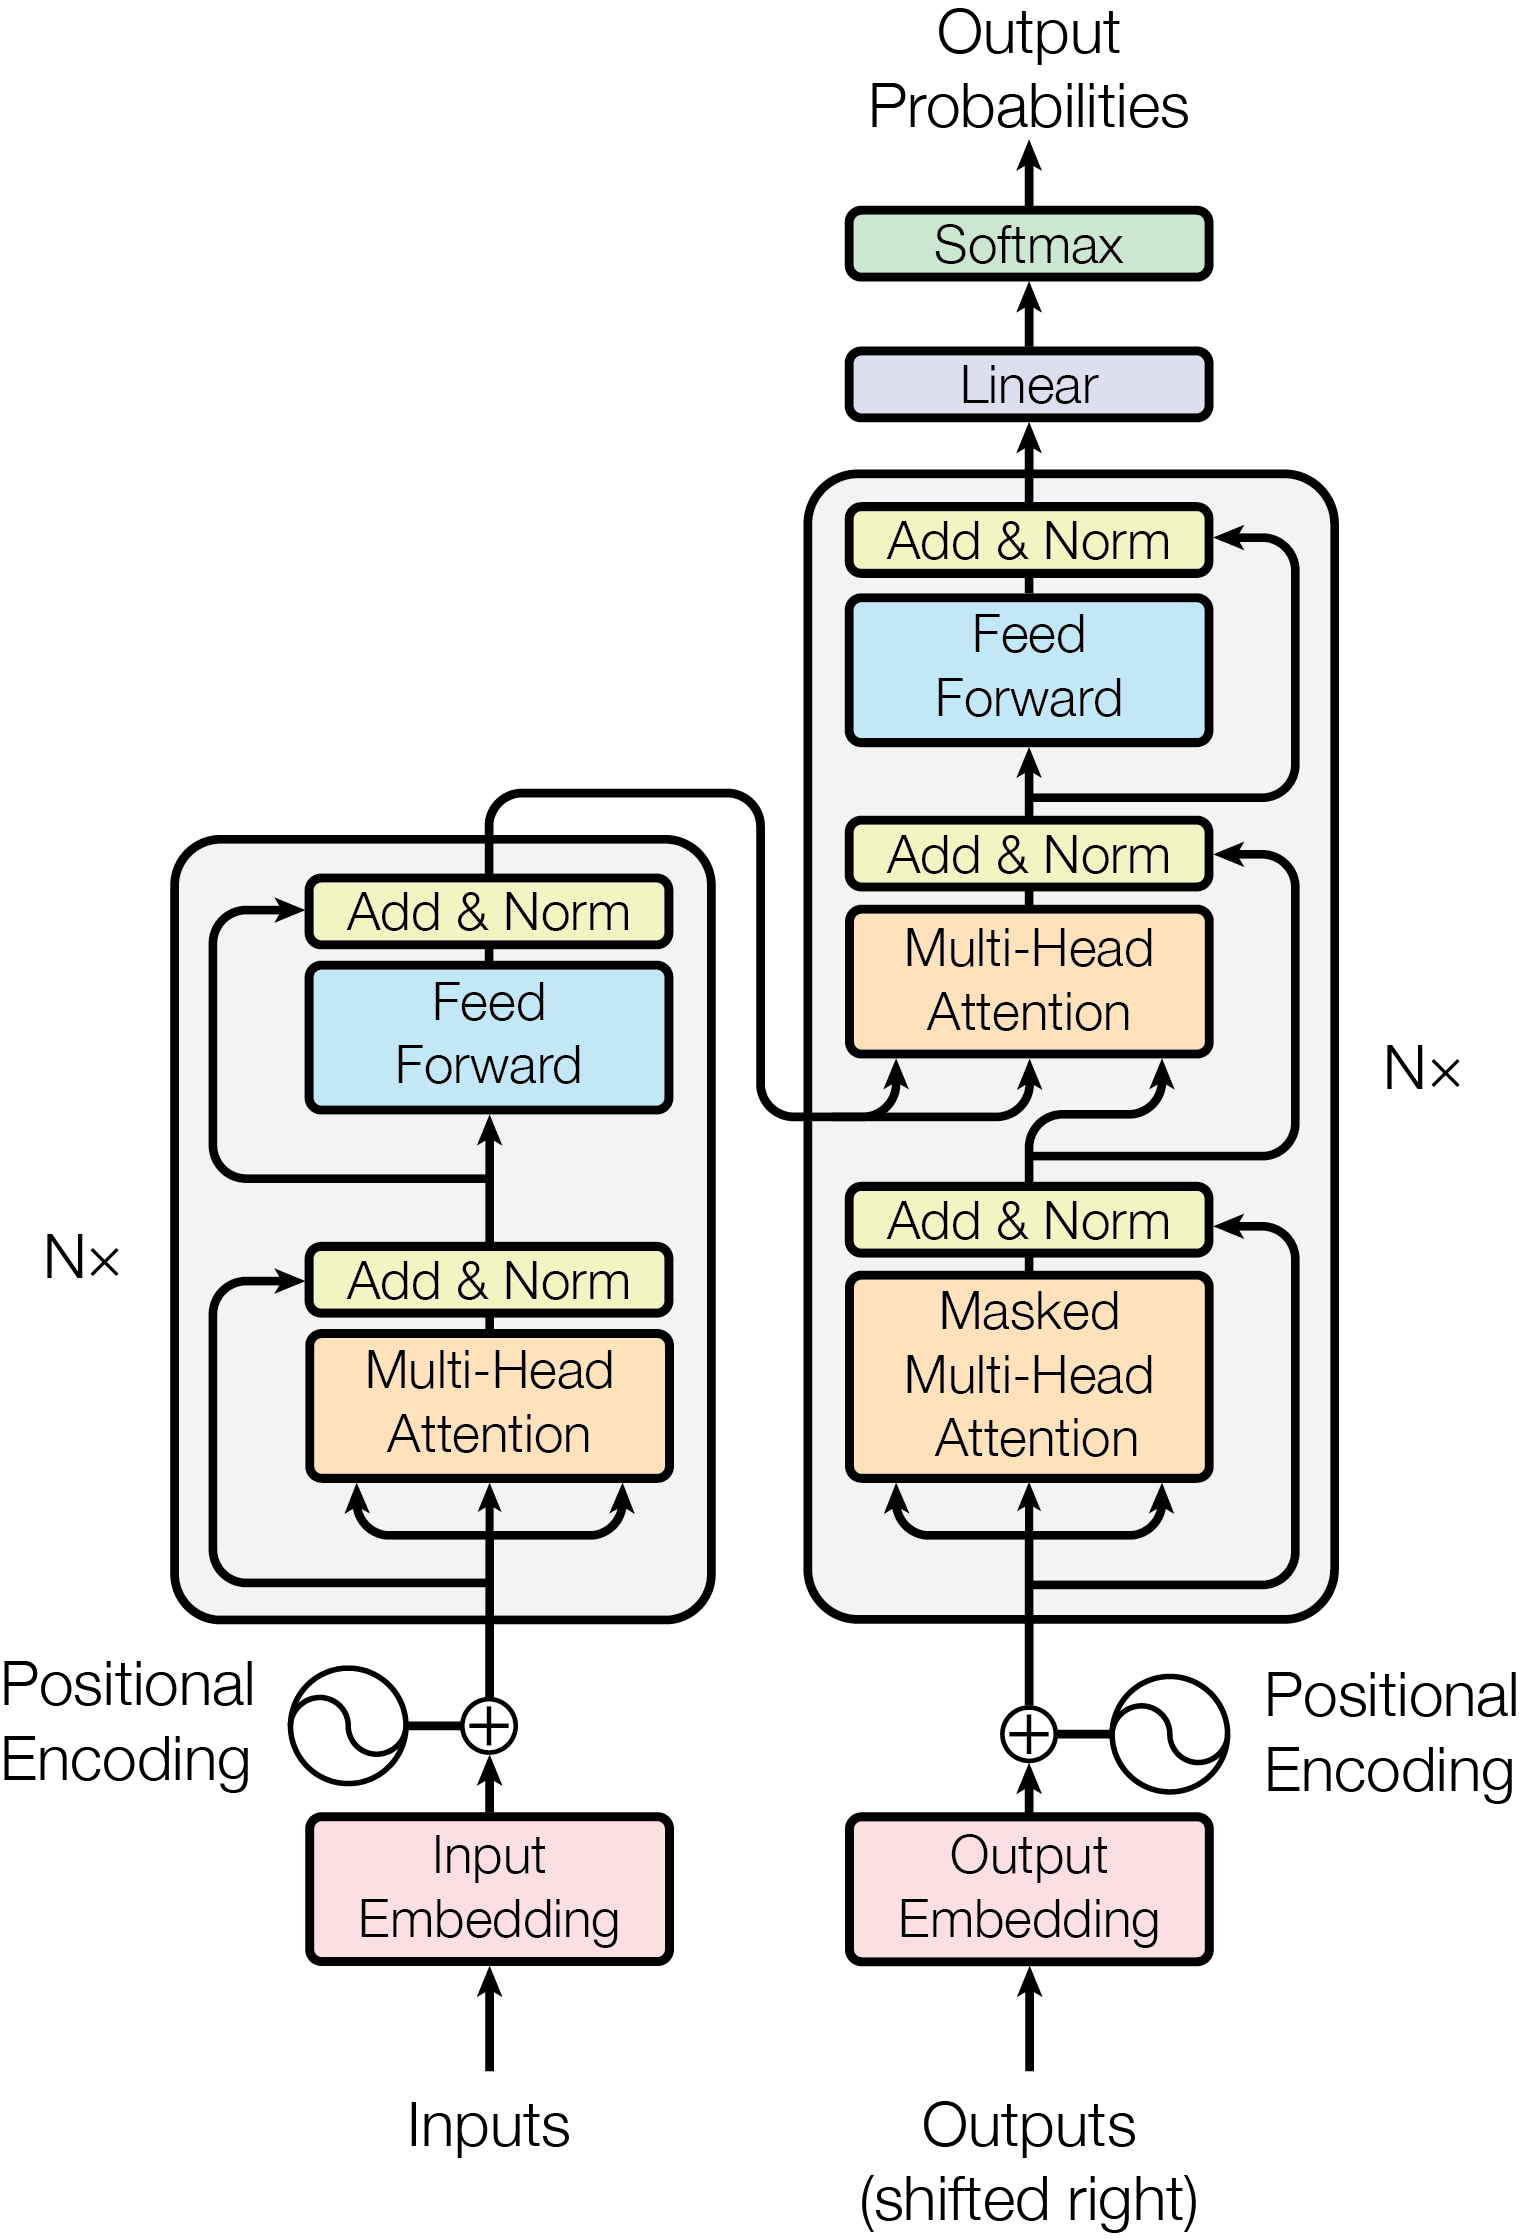
\includegraphics[width=0.7\linewidth]{images/transformerarchitecture.png}
	\caption{The Transformer model architecture. Image from \cite{transformer}.}
	\label{fig:transformerarc}
\end{figure}

More specifically, the Transformer's encoder  is composed of a stack of $N = 6$ identical layers. Each layer has two sub-layers: the first is a multi-head self-attention mechanism, and the second is a simple, position-wise fully connected feed-forward network. The authors added a residual connection (like ResNet \cite{resnet}) around each sub-layer, followed by layer normalization. The output of each sub-layer is $\text{LayerNorm}(x + \text{Sublayer(x)})$. The decoder is also composed of a stack of $N = 6$ identical layers. Each of them has the same sub-layers of the encoder with a third one which performs multi-head attention over the output of the encoder stack. The authors modify the self-attention
sub-layer in the decoder to prevent positions from attending to subsequent positions. This masking, combined with fact that the output embeddings are offset by one position, ensures that the predictions for position $i$ can depend only on the known outputs at positions less than $i$.

DETR \cite{detr} uses a standard Transformer developed for natural language process as proposed in \cite{transformer}. The high-level activation map $f$ extracted form the CNN backbone is rescaled form $C$ to a smaller dimension $d$ by a $1\times1$ convolution. The new feature map fed into the Transformer's encoder is $z_0 \in \R^{d, H, W}$. Since the encoder expects a sequence as input, the feature map $z_0$ is collapsed the spatial into one dimension, resulting in a $d\times HW$ feature map. The decoder transforms $N$ embeddings of size $d$.  The difference with the original Transformer \cite{transformer} is that DETR decodes the $N$ objects in parallel at each decoder layer. These input embeddings (called \textit{object queries}) are positional encoding vectors learned by the model during the training phase. They are passed to the input of each attention layer. Since the decoder is permutation-invariant, the $N$ input embeddings must be different to produce different results. Each object queries is transformed into an output embedding by the decoder. The number of object queries is an hyper-parameter and it must be greater that the quantity of different objects in an image.

\paragraph{Feed-Forward Networks} The $N$ object queries produced by the decoder are  independently classified into box coordinates and class labels by
a feed forward network, resulting $N$ final object predictions. The final predictor is composed by a 3-layer perceptron and a linear projection layer. The perceptron predicts the normalized center coordinates, height and width of the bounding boxes while the linear layer predicts the class labels. Since DETR predicts a
fixed-size set of $N$ bounding boxes, where $N$ is much larger than the
actual number of objects of interest in an image, an additional special class label $\varnothing$ is used to represent that no object is detected within a slot (it indicates the ``background'' class).

\subsubsection{DETR Loss Functions}
\label{sec:detrlosses}

DETR \cite{detr} simplifies the detection pipeline by dropping multiple hand-designed components that encode prior knowledge, like spatial anchors or non-maximal suppression. To address set prediction in a fully end-to-end way, DETR uses a novel loss function, called object detection set prediction loss, that produces
an optimal bipartite matching between predicted and ground truth objects, considering both the class labels and the bounding boxes.

\paragraph{Object detection set prediction loss} DETR \cite{detr} infers a fixed-size set of $N$ predictions through the $N$ object queries produced by the Transformer's decoder. It is important that $N$ is set to be significantly larger than the typical number of objects in an image. One of the main difficulties of training is to score predicted objects (class, position, size) with respect to the ground truth. The authors propose a loss function that produces
an optimal bipartite matching between predicted and ground truth objects, and
then optimize object-specific (bounding box) losses. 

\begin{figure}[h!]
	\centering
	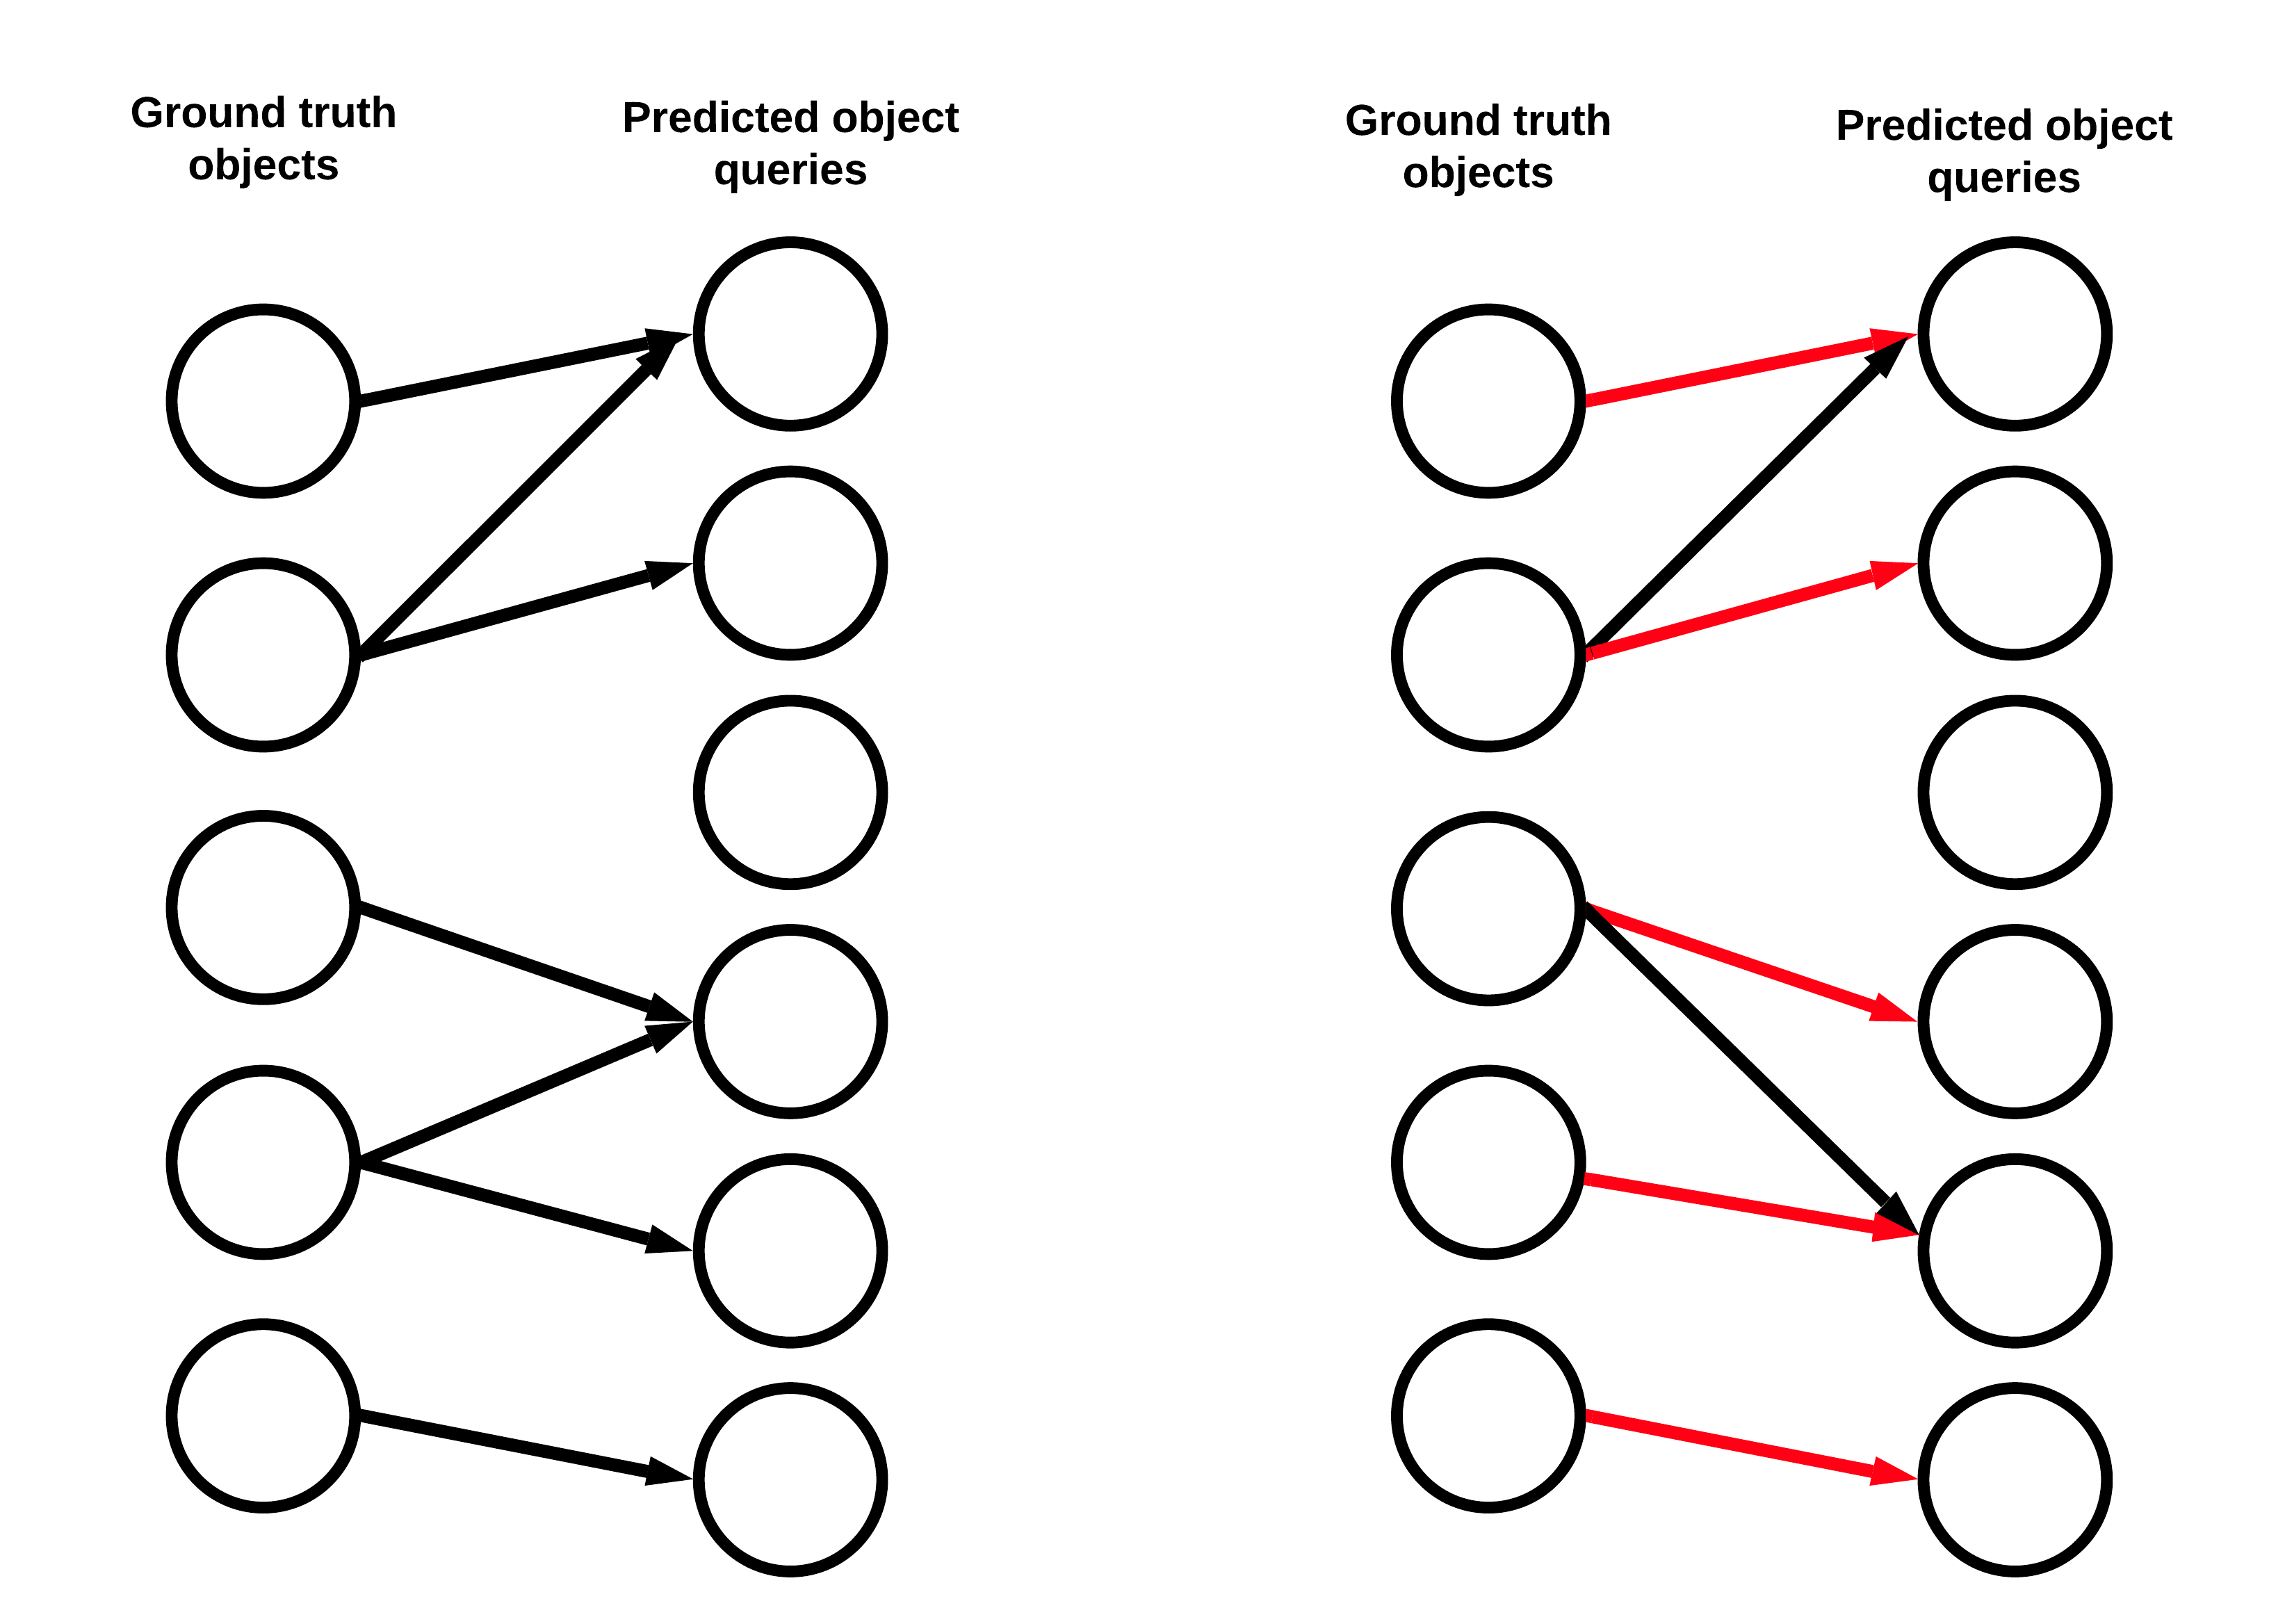
\includegraphics[width=0.6\linewidth]{images/bipartitematching.png}
	\caption{The Transformer model architecture. Image from \cite{transformer}.}
	\label{}
\end{figure}